%------------------------------------------------------------------------------
% This is a LaTeX template for the scientific justification of IRAM Proposals 
%------------------------------------------------------------------------------
% 
% We encourage IRAM proposers to use this template for the sake of unity 
% and clarity when Program Committee members assess their proposals.
% 
% You may customize this template to suit your preferences (e.g. using BibTex),
% but please respect the following requirements:
%     The scientific and technical justification should contain a 
%     maximum of 2 pages of text (4 pages for Large Programs), 
%     plus 2 pages of Figs., Tables and Refs.
%     Don't mix text with figures, tables, and references !!
%     The font size should be 11pt or larger.
%
% For Large Programs, the following sections should be included: 
%   i) Scientific Rationale, 
%  ii) Immediate Objective, 
% iii) Feasibility and Technical Justification, and 
%  iv) Organizational Issues.
%
%
%------------------------------------------------------------------------------
%
\documentclass[11pt,a4paper,twoside,graphicx,color]{article}
%
\usepackage[margin=2cm]{geometry}
\usepackage[pdftex]{graphicx}
\usepackage{color}
\usepackage{txfonts}
\usepackage{paralist}
\usepackage{amssymb}
\usepackage{lscape}
%
% Page size and text dimensions
% Do not change!
\textheight 260mm
\textwidth 178mm
\oddsidemargin -8mm
\evensidemargin -8mm
\marginparwidth 50pt
\topmargin -22mm
\brokenpenalty=10000
\sloppy
%-------------------------------------------------------------------
% command to emphatize the text (uncomment your preferred one)
%\newcommand{\emp}[1]{{\bf #1}}
\newcommand{\emp}[1]{\emph{#1}}
% Laurence's comments
%\newcommand{\laurence}[1]{\textcolor{blue}{#1}}
\newcommand{\laurence}[1]{#1}
%-------------------------------------------------------------------
\begin{document}
%
%
\begin{center}{\huge \bf
%-------------------------------------------------------------------
High-resolution tSZ observations of a large sample of clusters of galaxies 
%-------------------------------------------------------------------
}\end{center}
%
\centerline{\bf P.I.: Fr\'ed\'eric Mayet \& Barbara Comis (LPSC Grenoble)}


\section{Scientific Rationale}
As the largest gravitationally bound objects in the Universe,
clusters of galaxies represent the last step of the hierarchical process of structure formation.
Their abundance in mass and redshift is a powerful cosmological probe, as it is sensitive to the primordial
density fluctuations and the expansion history and matter content of the Universe.

In a cluster, most of the baryons are present within a gas that is hot
(10$^6$ - 10$^8$ K), diffuse and completely ionized. It is referred to
as the Intra-Cluster Medium (ICM). Cosmic Microwave Background (CMB)
photons may interact, via inverse-Compton scaterring, with the free hot
electrons in the ICM, being then shifted to higher energies.
This interaction, known as the thermal Sunyaev-Zel'dovich (tSZ)
effect, results in a CMB flux decrement (increment) at frequencies
below (above) $217~\rm{GHz}$.
%, which corresponds to a distortion of the CMB blackbody spectrum. 
The tSZ brightness   is proportional to
the integral of the electronic pressure   along the line
of sight ($\rm{y} \propto \int P_{e}\, dl$). Measuring the distribution of
the tSZ signal in clusters directly probes the distribution of thermal
pressure within the ICM. Furthermore, the tSZ flux is not affected by redshift cosmic dilution
as it is a CMB spectral distortion. Thus, the tSZ effect represents
a   well-suited observable to detect and study
clusters at high redshift ($z>0.4$), where their number and
distribution is the most sensitive to the underlying cosmology \cite{Carlstrom2002}.

In the last few years, technological progresses have made possible 
the detection of the tSZ effect routinely. As a consequence, tSZ-selected
cluster catalogues containing several thousands of candidates have been produced, at arcmin resolution, by the South Pole
Telescope (SPT, FWHM $\sim$ 1.1 arcmin at 150 GHz,
\cite{Reichardt2013, Bleem2015}), the Atacama Cosmology Telescope
(ACT, FWHM $\sim$ 1.4 arcmin at 148 GHz, \cite{Hasselfield2013}), and 
the Planck satellite (FWHM $\sim$ 10 arcmin for tSZ, \cite{PSZ1PSZ2}).   
However, their relatively limited resolution  only enables detailed study of the
spatial distribution of the signal for nearby clusters. ICM tSZ flux  ($\rm{Y}$) provides a
powerful tool for cosmological investigation with clusters, as long as
we are able to convert them into robust  estimates of the cluster total mass (M$_{tot}$).
At present, the systematic uncertainties ({\it e.g.} astrophysical systematics) affecting the mass-observable scaling relations 
represent the limit for cluster-derived cosmological constraints~\cite{PSZ1PSZ2}. 
Measurements reaching sub-arcminute angular resolution 
%for cluster pressure profiles 
are thus a mandatory step for
precise cluster  cosmology, since they will contribute to
improve our knowledge of the statistical properties of galaxy cluster
structure, by reducing the related uncertainties and biases.
 

%Such measurements can only be made   by high sensitivity and high spatial resolution tSZ observations. 
The NIKA2 camera at the IRAM
30~m telescope is the only instrument currently in operation that is
suited for this kind of observations and follow-ups, given its
resolution, sensitivity and dual-band observation capability. Conducting sub-arcminute tSZ observations of
a representative population of clusters across the almost unexplored
redshift range \laurence{$0.5 \lesssim z \lesssim 0.9$} will bring detailed insight of the
properties of clusters over more than 3 Gyr. This will allow us to
understand the processes driving the physical evolution of massive
halos in the Universe and to quantify how the cluster thermal content
and distribution evolves as massive halos   grow through
accretion and merging processes. This will
result in a better characterization of the mass-observable scaling
relations and its potential redshift evolution  within a  range relevant for   the precision of cluster-based cosmological studies. In short, the proposed LP sample will enable
a major breakthrough in the use of clusters of galaxies for
cosmological studies.


\section{Immediate Objective}
The main objective of this program is to obtain {\bf high resolution}
tSZ observations for a sample of objects, which are
{\bf representative} of the population of clusters of galaxies, at
{\bf intermediate and high redshifts (z $>$ 0.5)} and spanning one 
order of magnitude in SZ signal and mass. These observations
will be used for an in-depth study of the evolution of cluster
physical properties across cosmic times. At present, cluster and tSZ
derived cosmological constraints are limited by our incomplete
understanding of the impact of the details of cluster astrophysics.
Thus, this study is mandatory to handle systematics and achieve 
precision cosmology with clusters.\\ 
%As discussed before, NIKA2 is well adapted to explore the cluster
%population at intermediate and high redshift, within r$_{500}$
%(self-similar scale).%and at r $>$ r$_{500}$ (non-equilibrium
%regions).
%
%We aim at characterizing the details of the tSZ signal distribution
%in clusters at z~$>$~0.5,  The complementary information provided by
%the NIKA2 follow-up will lead to better understand and quantify the
%systematic uncertainties that might affect blind tSZ surveys (such as
%detection biases, constraining typical SZ profiles).
\laurence{Our first objective is to produce, for the whole selected cluster sample, unprecendented
  high-quality deliverables, such as tSZ maps and pressure profiles (see. Fig. \ref{Fig:CL_and_PSZ1}),  
   which we will release to the cosmology and astrophysics communities.} Then, we will characterize statistically the 
   properties of this high-redshift cluster population, by:

i) Exploring and test the regularity of the cluster pressure profile
at $z>0.5$, following the approach that has been used in X-rays with
the REXCESS sample at $z<0.2$ \cite{Arnaud2010}, but with an
observable (the SZ signal) that probes directly the ICM pressure.
%Is the pressure the quantity less affected by the cluster dynamical
%state and thermodynamic history? Is the SZ flux a robust mass proxy?
The major issue is the study of the mass-observable
scaling relation and its evolution with the redshift and the cluster
dynamical state.

ii) Detecting the presence of sub-structures ({\it e.g.} secondary peaks,
deviations from spherical symmetry, overall irregular shape), their
significance and impact on the global Y estimate.

iii) Introducing, defining and testing parameters that allow us to
quantify the cluster dynamical state through its tSZ morphology and fluctuations \cite{Khatri:2016jpa}. A
robust tSZ-defined indicator of cluster morphology would permit to
study the disturbed cluster fraction as a function of redshift and
would represent a useful tool to explore its correlation with
deviation from the cluster self-similar behavior observed at low $z$
and in hydrodynamical simulations for both the pressure profile and scaling laws, 
so linking the deviation from the mean to the (thermo-)dynamical history. 
	
iv) Studying the correlation between the SZ indicator(s) of cluster
dynamical state, the dispersion around the average cluster pressure profile
and its evolution with redshift and radial scale.  

This information is essential for  understanding cluster formation physics and performing precise  cosmological analysis with the cluster population.  Of particular importance is the clarification of  the physical origin of the normalisation, scatter and evolution  of the scaling relations,   particularly the mass- SZ observable relation, rendering their empirical calibration and their ultimate cosmological application more robust. The statistical properties of the pressure profiles, in link with the cluster dynamical states,  are also a key element for understanding the selection function of the SZ survey. 
%It is now clear that the latter must be fully mastered in order to understand the properties of the underlying population, and for cosmological applications (e.g. Angulo et al. 2012). The selection function depends not only on global properties (i.e. the link between the observable and the mass and its dispersion), but also on the profile properties (e.g. current SZ detection methods generally assume a given  pressure profile shape).

%\subsection{Feasibility and Technical Justification}

\section{Feasibility and Technical Justification}
The NIKA2 camera %is particularly well adapted
\laurence{represents a technological breakthrough} 
for high-resolution observations of the tSZ effect from cluster of
galaxies:

-- It \emp{operates simultaneously at two frequency} bands, $150$ and
$260~\rm{GHz}$, at which tSZ shows up respectively as a negative and a slighlty positive
distortion of the CMB spectrum, producing a very distinctive cluster
signal on the observed maps. For NIKA2, the main SZ signal is expected at 2 mm, while the 1mm band will be used for atmospheric and
point-source removal.
With NIKA, we have shown that dual-band observations can be used to
remove the atmospheric noise without affecting the signal, see \cite{Adam2014,Adam2015,Adam2016,Adam2016a,Ruppin2016}.
%taking advantage of the characteristic tSZ spectrum
In addition they are of the outmost interest to detect foreground
contaminating sources, and account for their flux.
%Both small and large angular scales may then be recovered. 
%with the price of a worse sensitivity. 


-- NIKA2 is made of \emp{arrays of thousands of high sensitive}
Kinetic Inductance Detectors (\emp{KIDs}). In particular we expect a
sensitivity in Compton parameter units of $\sim$~10$^{-4}$ per hour
and per beam. This should allow us to obtain reliable tSZ detections
and mapping of clusters of galaxies in few hours.

-- NIKA2, \emp{coupled to the IRAM 30 m telescope} allows us to map
clusters of galaxies to a \emp{resolution of typically $20~\rm{arcsec}$
  within a $6.5~\rm{arcmin}$ diameter FOV}.
%This is well adapted for medium and high redshift clusters for which
%we expect typical angular sizes of about 6-11 arcmin.
%(Figure \ref{Fig:size}).
%\vspace{0.1cm} 

NIKA2 tSZ capabilities have been demonstrated through a pilot study
conducted with its pathfinder, NIKA. In order to validate the KIDs capabilities when dealing with
such a faint and diffuse signal, we have mapped the tSZ in the
direction of six clusters of galaxies:
{\bf i)} RX~J1347.5-1145, an intermediate redshift object ($z=0.45$),
which has been the perfect target for the first tSZ detection ever
achieved with KIDs \cite{Adam2014};
{\bf ii)} CL~J1226.9+3332, a very high redshift cluster, $z=0.89$ \cite{Adam2015}, 
{\bf iii)} MACS~J0717.5+3745, which has been used to report the first
model-independent mapping of the kinetic Sunyaev-Zel'dovich
\cite{Adam2016};
{\bf iv)} MACS~J1423.9+2404, a relaxed cluster, which has been used to
explore the impact of the presence of foreground radio and IR sources
and how to deal with them in the data reduction \cite{Adam2016a};
{\bf v)} PSZ1~G046.13+30.75 and PSZ1~G045.85+57.71, two
Planck-discovered clusters (at $z=0.57$ and $z=0.61$, respectively) chosen
to test NIKA2 capabilities at the level of detection of the Planck
catalogue of tSZ sources \cite{Ruppin2016}.
We have   successfully explored a wide range of cluster morphologies and amplitudes of the tSZ flux. \\
%\vspace{0.3cm} \noindent {\bf \large Comparison with other high-angular resolution tSZ facilities -- } 
%It is important to compare NIKA2 to other existing and planned
%instruments for high resolution tSZ observations.
The MUSTANG and Bolocam instruments (at the focus of the
Green Bank Telescope and of the Caltech Submillimeter Observatory,
respectively) have also produced high quality tSZ
observations. They are expected to be followed by next generation
instruments. MUSTANG-2 represents the closest
NIKA2 concurrent instrument, even if it will not dispose of simultaneous dual-band capability, together with 
the next instrument on the LMT (BolocamII, TOLTEC), that will not be ready before NIKA2. As an alternative to large diameter telescopes,
interferometers can reach very high angular resolution, but they
cannot recover the large scale signal and they are time expensive (see Kitayama 2016 and Basu 2016).\\


%\vspace{0.1cm} 
\noindent  {\bf \large Target selection -- }
Our target selection strategy is mainly driven by the need of
selecting {\bf a sample of objects that is representative of the
  cluster population}.
%A flux-selected subset of a tSZ-selected catalogue can be considered
%as representative of a sample that is not biased towards a given
%morphology.
%\emp{As we want to derive relations that can be applicable
%  to the  whole cluster population} (not only relaxed or unrelaxed
%ICM) \emp{in order to achieve a global characterization of clusters
%  and an improved control of systematics due to their astrophysics}.
\laurence{A representative sample, {\it i.e.} which is not biased towards a given
cluster morphology, will allow us \emp{to derive mass-observable
  scaling relations that can be applicable to the whole cluster
  population} (not only relaxed or unrelaxed ICM) and \emp{to achieve
  a global characterization of clusters and an improved control of
  systematics due to their astrophysics}. A flux-selected subset of a
tSZ-selected cluster catalogue fulfills the requirement of a
representative sample.}
%
This criterion follows
%in fact
the approach adopted to build the REXCESS sample, an XMM-Newton large
program dedicated to the in-depth study of a representative sample of
33 X-ray selected clusters (0.055 $<$ z $<$ 0.183). This sample has been used to
build the universal pressure profile for the ICM \cite{Arnaud2010}, an
average profile for the cluster population, derived from observations,
scaled by mass and redshift according to the standard self-similar
model.
The LP SZ sample can be used to continue the  
characterisation of the cluster statistical properties, further
pushing the assessment of the potential evolution of the pressure
profile to higher redshifts, where X-ray observation becomes time consuming.

In order to fulfill our goal with NIKA2, we consider the following
main target selection criteria:

-- clusters belonging to tSZ-selected samples (already existing tSZ
based cluster samples from Planck and ACT), for which the redshift
information is available;

-- $0.5 < z < 0.9$, to explore the cluster statistical properties
beyond the local Universe;

-- $\rm{dec} > -11$, to ensure observability of the sources from the Pico
Veleta site.

%\vspace{0.1cm} 


%The current status of the follow-up observations of tSZ discovered Planck clusters (not fully completed) does not allow us to present a definitive catalogue of clusters of galaxies. However, 
We have used the above criteria and the Planck and ACT cluster samples to select a representative sample of clusters of galaxies suitable for our purposes. 
We note however that the external validation of the tSZ-discovered-Planck clusters is not yet fully completed.
%(Tab. \ref{tab:ACT_sample} and \ref{tab:PSZ1_sample}). 
We consider two bins in redshift (0.5~$<$~z~$\le$~0.7 and 0.7~$<$~z~$\le$ 0.9),
and for each of them, we have defined 
five bins in E$_z^{-2/3}$D$_A^2$Y$_{500}$ (Fig. \ref{Fig:CL_and_PSZ1}, bottom panel), which is the 
quantity related to the cluster mass M$_{500}$ through the scaling relation we aim at calibrating (D$_A$ is the angular diameter 
distance and E$_z$~=~H(z)/H$_0$ accounts for the background universe evolution). Within each bin we have selected 5 clusters maximising, when possible, the 
overlap with the SZ  clusters already planned for X-ray follow-ups with XMM-Newton (large programs PI: M. Arnaud). 
In summary, we have selected 45 out of 50 clusters and the  selected sample is listed in Tab. \ref{tab:selected_sample}. 
Note that we have added to the sample 
two extra clusters (backup) at high redshift  (see Table~\ref{tab:selected_sample}), to account for 
the large uncertainties in the definition of the properties of high redshift clusters.
For the two largest  E$_z^{-2/3}$D$_A^2$Y$_{500}$ bins (massive clusters) at high redshift we have at 
present only 4 and 1 cluster respectively. So, in agreement with IRAM, the remaining five clusters will be defined within one year from the starting of the large program. 
For this purpose, we will take advantage of the information  provided by current and near-future Planck and 
ACT follow-up programs, which are expected to populate the z $>$ 0.6 region.\\ 
 

%Therefore we have selected only 45 clusters for a total of about 210 hours. We expect these 5 clusters to account for less than 10 hours of observing time. Then, in total, we will need 220 hours of on source observations. Finally, 50 hours will be dedicated to calibration. We have also reserved a total of 30 hours (10 \% of the total) for possible loss of data due to bad weather, for example. In Tab.~\ref{tab:selected_sample}, in which we also list the last two objects of the XMM LP at $z~>$0.7 that have not been selected for the NIKA2 sample at this stage, but which fulfill our redshift and observability criteria. 


%\vspace{0.1cm} 
\noindent {\bf \large Observing strategy and data reduction -- } Based on the experience with the NIKA camera, we will 
perform OnTheFly (OTF) scans in right ascension and declination. We will alternate different 
orientations of the scans (e.g. 0, 45, 90,-45 degrees) and perform scans of 13' $\times$ 8'. Hence, 
more than one third of the observing time will be spent on the core of the signal. This will allow us to properly define the zero level of the final map and measure angular scales structures up to the scan size. %Smaller scans of 11' $\times$ 7' will be considered in the case of high redshift and low mass clusters ($\theta_{500}$ $<$ 2.25 arcmin). 
To estimate the expected cluster signal in the maps we use the Y$_{500}$ (Y$_{500} =  \int_{\Omega_{r_{500}}}y d\Omega$), M$_{500}$ and redshift provided from the latest updated version of Planck 
and the   cluster catalogs. We then consider an universal pressure profile \cite{Arnaud2010} to model the distribution of the signal around the cluster center for 
each   Y$_{500}$. The required observation time are optimized cluster by cluster, in order to obtain an homogeneous sample in terms of signal to noise at a given characteristic radius $\theta_{500}$ (radius at which the cluster mean over density is equal to 500 times the critical density of the Universe). 
We impose at least a 1-$\sigma$ measurement of the cluster pressure profile at $\theta_{500}$ (see. Fig. \ref{Fig:CL_and_PSZ1}) 
for all clusters in the sample. Notice that the $\theta_{500}$ is computed from the redshift and the tSZ-derived M$_{500}$ reported in the catalogues, in order to have a homogeneous definition that only depends on the tSZ flux and the cluster distance. 


Transforming the above criteria into a rms noise in the map we compute the observing time per cluster using the NIKA2 time estimator provided by IRAM. We consider millimetre weather 
conditions with 2 mm of PWV, an overhead factor of two, 60 \% of valid detectors and a conservative filtering of about 30 \% within the cluster characteristic radius. The expected observing time per cluster are presented in Table~\ref{tab:selected_sample}. We also specify that we have used the $y$ to Jy/beam conversion reported in \cite{Adam2015}. Roughly speaking we require observing times of 
about 10 to 20 hours for 
the faintest clusters and of 1-3 hours for the most massive ones. 
To provide an example, by re-projecting the Planck flux for the NIKA observed cluster PSZ1~G045.85+57.71, we obtain an expected tSZ peak at $\sim$2~mJy/beam (consistently with what shown in \cite{Ruppin2016}). And we recall here that, for this cluster, 4.3 hours of observation with the NIKA prototype allowed a map quality comparable to what we require in this program (allowing a non parametric pressure profile deprojection 
up to $\theta _{500}$, Fig.~\ref{Fig:CL_and_PSZ1}, upper right panel). In the PSZ catalogue, this cluster has close properties to PSZ2~G046.13+30.72, for which we require 4 hours of observation. 
For the 45 selected clusters 
we obtain a total observing 
time of 280 hours. The total time on pms is 287 as it accounts for the two backup clusters that may replace two clusters of the sample if
needed.  The remaining 20 hours will be used to accommodate the observations of the lacking five high mass clusters. 
In the case of improved instrument performance we intend to keep the same number 
of sources and the same integration time for each of them, in order to extend morphology analysis out to the cluster outskirts.  
To illustrate, in the case of goal performance and 
30\% of overhead time (as reached during NIKA observations), the signal to noise will be improved by a factor of about 2.5.

% To estimate the observing time needed per cluster we have performed simulations including signal, as just discussed, and noise. In terms of noise we have considered simulations taking the NIKA2 specification sensitivity at 2$~$mm of 20 mJy/beam/s$^{1/2}$, and increased the noise by 30 \% to account for correlated noise extra variance. In addition, we have considered the real FOV of the instrument (6.5') and a FWHM of 20'' at 2$~$mm. By contrast we have considered no atmospheric contamination and uniform weather conditions across the sample. 
%As one of the major objectifs of the project is to have a clear picture of the morphology of the clusters we need to set strong requirements on the signal-to-noise at the map level to ensure structures
%are significantly detected at least up to $\theta_{500}$. As we expect the SZ signal to peak towards the center of the cluster this criteria also ensure significant detection in the inner part of the cluster.
%Assuming a perfect reconstruction of the cluster up to $\theta_{500}$ (no filtering) and requiring 4$~\sigma$ detection at $\theta_{500}$ on the map for pixels of the size of the beam, we can compute the needed observing time per cluster.  In addition we also impose a minimum of 1 hour of integration per cluster to ensure sufficient  scan redundancy.  If the final instrument performance are improved with respect to the specifications we plan to keep the same number of clusters as well as of the same observation time per cluster in order to recover large scale structures beyond $\theta_{500}$.


In terms of data reduction we will use the tSZ dedicated pipeline developed for the NIKA experiment. This pipeline has beed intensively tested
using the NIKA data and was used for the NIKA SZ publications \cite{Adam2014,Adam2015,Adam2016,Adam2016a,Ruppin2016}. 
Needed improvements and updates will be directly carried out by our team that  led the analysis of the NIKA SZ data.
NIKA2 will be able to observe simultaneously at two wavelengths allowing for self consistent foreground source subtraction 
(e.g. \cite{Adam2016a}). 
However NOEMA could be eventually
used to obtain complementary information in this sense, requiring
reasonable observing times.

\section{Organizational Issues}

%\vspace{0.1cm} 
\noindent{\bf \large Project management -- } For this project we have
gathered a highly experienced team with a large expertise in
submillimetre observations, data reduction and tSZ science as well as
complementary external observations. A project PI (F. Mayet) and a
co-PI (B. Comis) will coordinate the different activities. As an
expert of the NIKA2 pipeline, the co-PI is in charge of coordinating
the data reduction, according to NIKA2 collaboration rules. The NIKA2SZ
team have a long experience of SZ data with NIKA observations,
together with external data for joint analysis. For the sake of
clarity, the team can be presented in two sub-teams:\\
\indent {\bf - NIKA2SZ analysis team} : R. Adam, B. Comis,  M. De
Petris, J.-F. Macias Perez, F. Mayet,  L. Perotto, C. Romero,
F. Ruppin. 
The NIKA2SZ analysis team has developped a SZ pipeline enabling the
processing from raw data to SZ maps and pressure profiles (Fig.~\ref{Fig:CL_and_PSZ1}), which are
the main deliverables of this LP. It has been tested and
optimized on observation with the NIKA intrument, leading to five
papers in the recent years
\cite{Adam2014,Adam2015,Adam2016,Adam2016a,Ruppin2016}.\\
\indent {\bf - NIKA2SZ ancillary data team}  :   M. Arnaud,
I. Bartalucci, G. Pratt, E. Pointecouteau (XMM group for X-rays),
J. A. Rubino Martin, R. Barrena Delgado (GTC team for optical
observations) and C. Ferrari (LOFAR team for radio emission). 
Experts of external data have contributed to the definition of the cluster
sample. Furthermore, to maximize the scientific output of the 
NIKA2SZ, they are participating in the joint analysis
with NIKA2 data. Also, follow-ups are being prepared for the near
future. Note that this team has contributed to the NIKA SZ papers,
proving the added value of external data
\cite{Adam2014,Adam2015,Adam2016,Adam2016a,Ruppin2016}.


%\vspace{0.1cm} 
\noindent {\bf \large Data policy and deliverables-- }  The  
data and products of the LP will be made publicly available by the NIKA2
collaboration in a dedicated database after the end of the LP
observations, following the standard IRAM rules. These products will
consist of the raw data, the calibrated map per cluster and associated
processing information, and pressure profiles per cluster.


%\vspace{0.1cm} 
\noindent{\bf \large Complementary external data -- } The scientific
output of the NIKA2 LP could be enriched by the use of high quality
external data at other wavelengths or with other probes. Other than
the use of publicly available data, formal collaborations are being
established to collect extra proprietary data. At this regard, XMM
data from a companion X-ray follow-up of high-redshift clusters will
be used. With NIKA2 the cluster gas will be finally mapped in tSZ with
a quality (in terms of sensitivity and angular resolution) comparable
to X-ray, even for intermediate and high-redshift clusters. Thus, the
natural combination of these two direct observables of the
intra-cluster hot gas will allow us
to estimate the total masses (under the assumption of hydrostatic
equilibrium) as well as a full physical characterization of the
(radial) distribution of the cluster thermodynamic properties: not
only pressure, but also temperature (T$_{e}$(r) $\propto$
P$_{e}$(r)/n$_{e}$(r)) and entropy (K(r) $\propto$
P$_{e}$(r)n$_{e}^{-5/3}$) which are essential to unveil cluster
thermodynamic history. Indeed, the tSZ signal directly probes the gas
pressure, while X-ray data deliver the gas density squared and
temperature. The different dependencies of tSZ and X on the electron
density will also provide a powerful probe of gas clumping, and an
improved insight on the cluster tridimensional shape.

Furthermore, optical follow-ups could be performed for a large number
of the NIKA2 clusters using the GTC (Gran Telescopio Canarias) imaging
and spectroscopy facilities. The combination of tSZ and X-ray data to
optical/NIR observations of the cluster galaxies will further help to
investigate the connection between galaxy properties (luminosity
function, SFR, stellar mass) and those of the ICM, and thereby bring
constraints on feedback mechanisms at play within clusters. Moreover,
weak lensing measurements will provide complementary measurements of
the dark matter distribution and total mass of the clusters, in a
totally independent way, then affected by different
systematics. Optical mass estimate are not based on the same
assumptions.
The thermodynamical and dynamical properties of the observed clusters will be compared  
with outputs from numerical simulations such as MUSIC \cite{sem14}.




%\section{Supporting material}
% You may include up to two pages of figures, tables, and References.

% Below is an example for including a figure in your proposal.
% If you are compiling with pdflatex, you can include jpeg, png, and pdf files.
% if compiling with latex, only eps files can be included. 
%\begin{figure}
%    \centering
%    \includegraphics[width=0.8\textwidth]{image.png}
%    \caption{Enter the figure caption here.}
%    \label{fig:myPlot_1}
%\end{figure}
%\begin{landscape}

\newpage




\begin{figure}[t]
  \centering
\hspace*{-1cm}   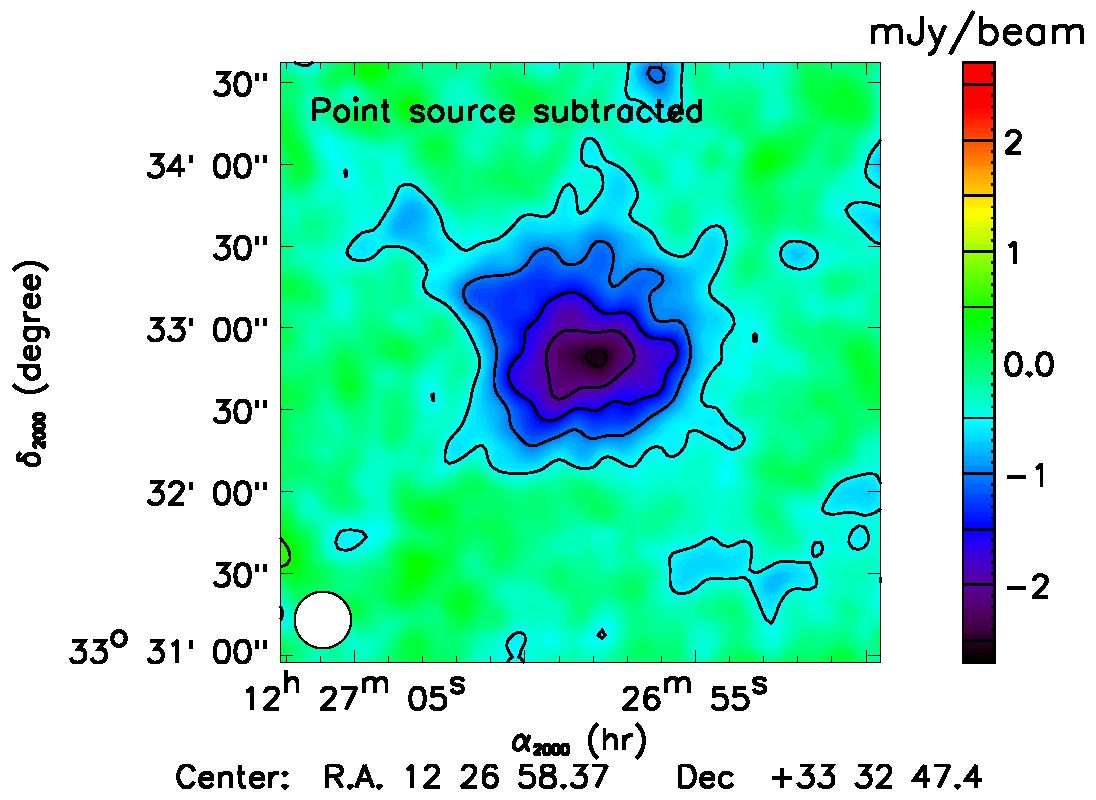
\includegraphics[scale=0.45]{./Figures/CL1226}
   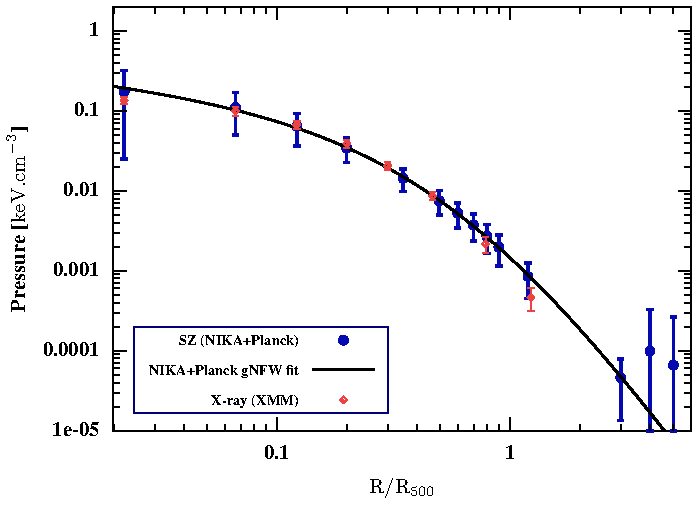
\includegraphics[scale=0.7]{./Figures/Pressurenonparam.pdf}
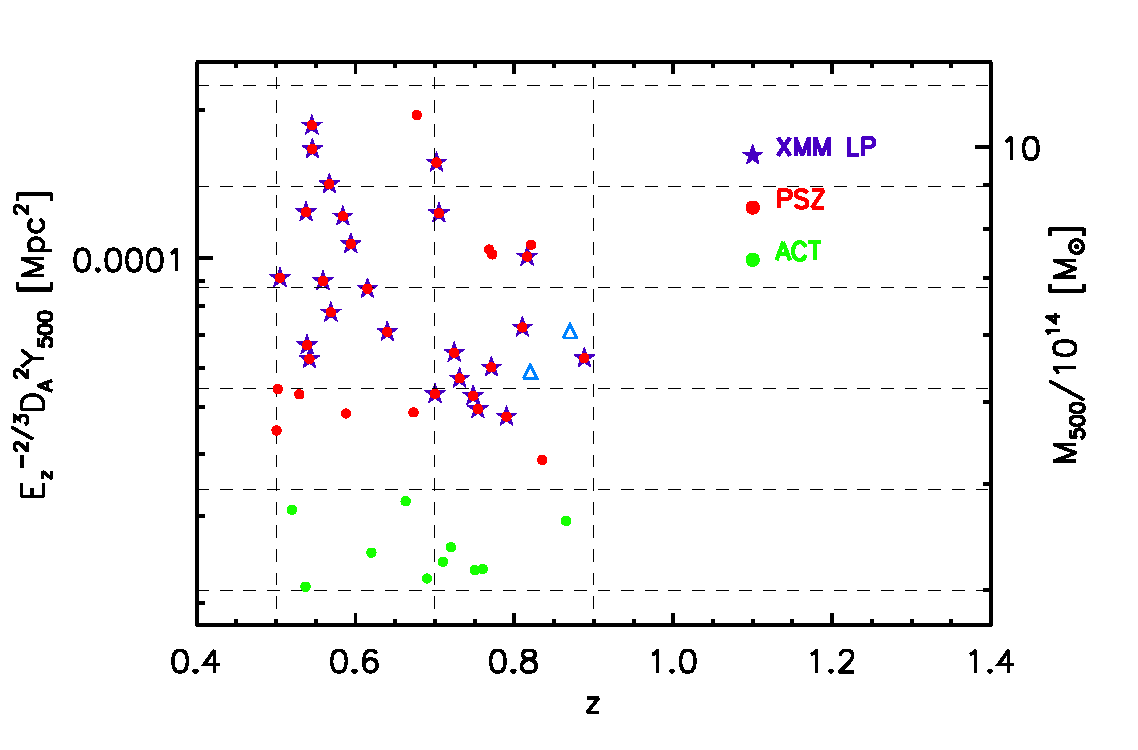
\includegraphics[scale=0.45]{./Figures/NIKA2_sample}   
\caption{{\small {\bf Upper Left:} NIKA map of CL J1226.9+3332 at 150 GHz \cite{Adam2015}. The effective beam FWHM (18.2 arcsec native resolution plus an extra 10 arcsec FWHM Gaussian) is shown as 
the bottom left white circle.  The overall effective observing time on the cluster is 7.8 hours and $\theta_{500} \sim 2~\rm{arcmin}$ for this cluster. 
{\bf Upper Right:} 
Non-parametric pressure profile (blue) deprojected from the 
NIKA tSZ surface brightness map of a Planck-discovered cluster 
(PSZ1\,G045.85+57.71) observed with NIKA in Oct. 2014. Fig.~from \cite{Ruppin2016}.
This   was part of a NIKA pilot study aimed 
at preparing the NIKA2 tSZ Large Programme. {\bf Bottom} : Clusters extracted from the Planck and ACT (equatorial) tSZ-selected samples, in the redshift range we want to explore 
and observable from the Pico Veleta site (dec $>$ -11). The different symbol used are reported in the legend, 
the cyan triangles are the two further objects belonging to the XMM large program (listed at the end of 
Tab. \ref{tab:selected_sample})}}
\label{Fig:CL_and_PSZ1}
\end{figure}



 

%\clearpage



\begin{thebibliography}{99}
 \bibitem{Carlstrom2002} {\small Carlstrom, J. E., Holder, G. P., \& Reese, E. D. 2002, ARA\&A, 40, 643}
   
 \bibitem{Reichardt2013}
   {\small Reichardt, C. L., Stalder, B., Bleem, L. E., et al. 2013, ApJ, 763, 127}
   
 \bibitem{Bleem2015}
   {\small Bleem, L. E., Stalder, B., de Haan, T., et al. 2015, ApJS 216, 27}
   
 \bibitem{Hasselfield2013}
   {\small Hasselfield, M., Hilton, M., Marriage, T. A., et al. 2013, J. Cosmology Astropart. Phys., 7, 8}
   
 \bibitem{PSZ1PSZ2} 
   {\small Planck Collaboration, A\&A, 571, A29, ArXiv:1502.01598, ArXiv:1502.01597, ArXiv:1502.01596}
 
 \bibitem{Arnaud2010}
    {\small Arnaud, M., Pratt, G. W., Piffaretti, R., et al. 2010, A\&A, 517, A92}
  
 \bibitem{Adam2014}
   {\small Adam, R., Comis, B., Mac{\'{\i}}as-P{\'e}rez, J.-F. et al. 2014b, A\&A, 569, A66}
 
 \bibitem{Adam2015}
   {\small Adam, R., Comis, B., Mac{\'{\i}}as-P{\'e}rez, J.-F. et al. 2015, A\&A, 576, A12}
   
 \bibitem{Adam2016}
 {\small Adam, R., Bartalucci, I., Pratt G. W. et al. 2016, ArXiv:1606.07721}
 
 \bibitem{Adam2016a}
   {\small Adam, R., Comis, B., Bartalucci, I. et al. 2016, A\&A, 586, A122}
   
 \bibitem{Ruppin2016}
   {Ruppin, F., Adam, A., Comis, B., et al. 2016, ArXiv:1607.07679, to appear in A\& A}

\bibitem{Khatri:2016jpa}
  R.~Khatri and M.~Gaspari, arXiv:1604.03106  
   
\bibitem{sem14}
  F. Sembolini, M. De Petris, G. Yepes, {\it et al.} (2014), MNRAS, \textbf{440}, 3520
  

\end{thebibliography}

 
 

\begin{table}
\centering
\resizebox{\textwidth}{!}{%
\begin{tabular}{|l  || c | c | c | c | c | }
  \hline                       
Name  & Alternative Name &  z  & $\theta_{500}$  & Y$_{500}$  & t$_{obs}$  \\ 
   & $ $ &    & [arcmin] & [10$^{-4}$ arcmin$^{2}$] &  [hr] \\ 
   \hline
  ACT-CL J0219.8+0022  &                                                                             &          0.537  &   2.169   &  1.700  &   21.7 \\%   0.215
  ACT-CL J2152.9-0114   &                                                                             &           0.690  &   1.820  &   1.500  &   16.9 \\%   0.224
  ACT-CL J0240.0+0116  &                                                                              &          0.620  &   2.022  &   1.800  &   16.0  \\%   0.253
  ACT-CL J2302.5+0002  &                                                                              &           0.520  &   2.381 &    2.500  &  13.9  \\%   0.309
  ACT-CL J0223.1-0056   &                                                                              &          0.663  &   2.023  &   2.200  &   11.0  \\%   0.321
  \hline
  PSZ2 G081.02+50.57   &     RMJ153906.4+503644.9                                  &           0.501 &    2.650  &   3.739  &   8.8  \\%   0.447
  PSZ2 G106.15+25.75   &     PSZ1 G106.15+25.76 					 & 		0.588  &   2.396  &  3.573  &    7.2  \\%   0.484
  PSZ2 G108.27+48.66   &     PSZ1 G108.26+48.66                                     &             0.673  &   2.185  &   3.304  &   6.3  \\%   0.487
  PSZ2 G133.59+50.68   &     RMJ114649.1+650506.8                                 &            0.529  &   2.626  &   4.228  &    6.8 \\%    0.530
  PSZ2 G080.64+64.31   &     RMJ142716.1+440730.6                                  &           0.502  &   2.741  &   4.523  &    6.8  \\%   0.543
  \hline 
  PSZ2 G212.44+63.19   &     PSZ1 G212.51+63.18, RMJ105252.4+241530.0, WHL J163.208+24.18        &       0.542  &   2.663   &  4.896  &   5.4  \\%   0.625
  PSZ2 G094.56+51.03   &     PSZ1 G094.54+51.01, RMJ150822.0+575515.2, WHL J227.050+57.90        &       0.539  &   2.706  &   5.244  &   5.0  \\%   0.667
  PSZ2 G193.31-46.13    &    PSZ1 G193.29-46.13, PLCK G193.3-46.1          &         0.640   &  2.426  &   4.957  &   4.0 \\%   0.710
  PSZ2 G046.13+30.72   &     PSZ1 G046.13+30.75, RMJ171705.5+240423.6        &     0.569  &   2.679  &   5.868  &   4.0  \\%   0.777
  PSZ2 G099.86+58.45   &     PSZ1 G099.84+58.45, WHL J213.697+54.78             &     0.615  &   2.589  &   6.213  &   3.2  \\%   0.868
  \hline
  PSZ2 G183.90+42.99   &     PSZ1 G183.92+42.99, RMJ091051.0+385022.4, WHL J137.713+38.83   &     0.559  &   2.788   &  6.884  &   3.3  \\%   0.900
  PSZ2 G211.21+38.66   &     PSZ1 G211.23+38.63, RXC J0911.1+1746, RMJ091111.5+174628.9	&         0.505  &   3.008   &  7.575  &   3.3  \\%   0.913
  PSZ2 G045.32-38.46   &     MACSJ2129.4-0741, RMJ212926.1-074127.9, J2129.4-0741                &          0.594  &   2.758   &  7.841  &   2.5  \\%   1.070
  PSZ2 G144.83+25.11  &      PSZ1 G144.86+25.09, MACSJ0647.7+7015, RXC J0647.8+7014         &          0.584  &   2.859  &   9.026  &   2.0  \\%   1.217
  PSZ2 G201.50-27.31   &     PSZ1 G201.50-27.34, MACSJ0454.1-0300, RXC J0454.1-0300             &          0.538  &   3.043  &   9.783  &   2.1 \\%   1.241
  \hline
  PSZ2 G155.27-68.42   &     PSZ1 G155.25-68.42, RMJ013725.0-082722.7, WHL J24.3324-8.477    &          0.567  &   3.002  &  10.711  &   1.7  \\%   1.415
  PSZ2 G111.61-45.71    &    PSZ1 G111.60-45.72, RXC J0018.5+1626, CL 0016+1609                      &          0.546  &   3.182  &  12.991  &   1.4  \\%   1.667
  PSZ2 G228.16+75.20   &     PSZ1 G228.21+75.20, RXC J1149.5+2224, RMJ114935.7+222354.6, MCS J1149.5+2223   &   0.545  &   3.250  &  14.522  &   1.3   \\%  1.862
  PSZ2 G209.79+10.23    &    PSZ1 G209.80+10.23                                         &   0.677  &   2.819  &  13.220   &  1.0   \\%  1.954
  \hline
  \hline
  ACT-CL J0018.2-0022    &                                                                               &      0.750   &  1.739   &  1.500  &   14.6  \\%   0.233
  ACT-CL J0058.0+0030   &                                                                               &      0.760   &  1.742  &   1.500  &   14.3  \\%   0.234
  ACT-CL J2130.1+0045   &                                                                               &      0.710   &  1.823  &   1.600  &   14.7   \\%  0.242
  ACT-CL J0119.9+0055   &                                                                                &      0.720  &   1.825  &   1.700  &   13.3  \\%   0.259
  ACT-CL J0215.4+0030   &                                                                               &       0.865  &   1.648  &   1.800  &   9.0   \\%  0.293
  \hline
  PSZ2 G104.74+40.42    &    PSZ1 G104.78+40.45                                         &       0.835  &   1.816  &   2.417  &   6.5   \\%  0.390
  PLCK G079.95+46.96    &                                                                                &      0.790  &   1.955  &   3.013  &   5.4   \\%  0.477
  PSZ2 G088.98+55.07    &    PSZ1 G089.04+55.07                                         &       0.754  &   2.029  &   3.178  &   5.5   \\%  0.495
  PSZ2 G087.39+50.s92    &    PSZ1 G087.32+50.92, AMF J231.538+54.13     &       0.748  &   2.064  &   3.393  &   5.0  \\%   0.526
  PSZ2 G097.52+51.70   &                                                                              &           0.700  &   2.162  &   3.530  &   5.4  \\%   0.531
  \hline
  PSZ2 G084.10+58.72    &    PSZ1 G084.04+58.75                                         &       0.731  &   2.128  &   3.717  &   4.7   \\%  0.571
  PSZ2 G086.93+53.18    &    PSZ1 G086.93+53.18, WHL J228.466+52.83     &      0.771  &   2.074  &   3.828  &   4.1   \\%  0.601
  PSZ2 G160.83+81.66    &    BVH2007 154, CL J1226.9+3332                        &      0.888  &   1.907  &   3.827  &   3.2   \\%  0.627
  PSZ1 G226.65+28.43    &    WHL J134.086+1.780                                          &      0.724  &   2.190  &   4.209  &   4.0   \\%  0.644
  PLCK G227.99+38.11    &                                                                                 &      0.810  &   2.079  &   4.532  &   3.1   \\%  0.724
  \hline
  PSZ2 G091.83+26.11    &    PSZ1 G091.82+26.11                                           &      0.816  &   2.200  &   6.298  &   2.0   \\%  1.009
  PSZ1 G140.10+50.09    &                                                                                  &     0.772  &   2.286  &   6.486  &   2.1   \\%  1.019
  PSZ1 G224.73+33.65    &    CXOMP J091126.6+05                                         &     0.768  &   2.303  &   6.647   &  2.0   \\%  1.042
  PSZ2 G141.77+14.19    &    PSZ1 G141.73+14.22, WHT                                 &     0.821 &    2.214  &   6.641  &   1.8   \\%  1.066
  PSZ1 G080.66-57.87     &   ACT-CL J2327.4-0204                                           &      0.705  &   2.518  &   8.182  &   1.8   \\%  1.235
  \hline
  PSZ2 G138.61-10.84     &   PSZ1 G138.60-10.85                                             &      0.702  &   2.639  &  10.395  &   1.3  \\%   1.566
  \hline
  \hline
  {\it PSZ2 G071.82-56.55}  &   {\it MEGACAM (redshift id)} &  {\it 0.870}   &  {\it 1.978}   &  {\it 4.358}  &   {\it 2.8}  \\%   0.711
  {\it PSZ2 G092.69+59.92}  &   {\it MEGACAM (redshift id)}  &  {\it 0.820}  &   {\it 1.984}  &   {\it 3.669}  &   {\it 3.9}  \\%   0.589
  \hline
\end{tabular}
}
\caption{{\small Clusters selected for the NIKA2 SZ large program. We report the Planck/ACT name 
of the object, the alternative names, the redshift, $\theta_{500}$, 
$Y_{500}$ and the estimated time. In italics, we list two backup objects from the XMM large program.}}
 \label{tab:selected_sample}
\end{table}
%\end{landscape}
%%%%%%%%%%%%

\end{document}
